\section{Evaluation}
It is important to validate my design to ensure its functionality. Here I discuss my test procedure, my findings, and my conclusions on how well my design meets the requirements. The architecture evaluated here is shown in Appendix~\ref{app:block_diagram}.

\subsection{Validating the FFT Accelerator}
After synthesizing the strided FFT from MachSuite~\cite{machsuite} in Vivado HLS, it was important to verify that the accelerator actually computed an FFT correctly. To proceed, the FFT accelerator's results must exactly match those of the FFT computed in software. My results show that these expectations are met---the FFT hardware accelerators compute exactly the same results as the FFT software.

\subsubsection{Methodology}
The results of each of the three FFT accelerators present in the architecture were compared against the results of the MachSuite C code in order to validate them. The MachSuite C code was copied and pasted into the Xilinx SDK where it was compiled for the Zynq processor. The Zynq processor then computed seven FFTs using the same inputs: one in software; the other six on each of the three hardware accelerator instances, either using a DMA engine or not. Results from each were checked for equality using the function in Listing~\ref{lst:validation_func}. The results of the hardware FFT are passed as arguments \texttt{real\_hw} and \texttt{img\_hw}, and the results of the software FFT are \texttt{real\_sw} and \texttt{img\_sw}.

\begin{lstlisting}[caption={FFT Validation Function},label={lst:validation_func}]
static void compare_results(double real_hw[FFT_SIZE], double real_sw[FFT_SIZE], double img_hw[FFT_SIZE], double img_sw[FFT_SIZE]) {
	int i;
	for(i=0; i<FFT_SIZE; i++){
		if(real_hw[i] != real_sw[i] or img_hw[i] != img_sw[i]) {
			xil_printf("ERROR: Different results at bin %d\n", i);
		}
	}
}
\end{lstlisting}

\subsubsection{Results}
No differences arose between the results of the software FFT and any of the hardware-accelerated FFTs. This means that all three hardware FFTs correctly implement the strided FFT algorithm.

\subsection{Examining Accelerator-Rich System Performance Relative to Software}
With the previous test, I showed that the FFTs compute the correct results. With this test, I demonstrate the usefulness of the DMA engine and clock scaling in improving the performance of the FFT in hardware versus in software.

\subsubsection{Methodology}
The FFT was re-synthesized using Vivado HLS with a target clock frequency of 120MHz. The timing portion of the C synthesis report is printed in Figure~\ref{fig:120mhz_syn_report}.
\begin{figure}
\begin{center}
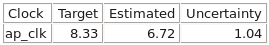
\includegraphics[resolution=100]{fft120_syn_report}\\
\end{center}
\caption{Timing characteristics taken from the C Synthesis Report for MachSuite's Strided FFT, generated by Vivado HLS. Targeting a clock frequency of 120MHz.}
\label{fig:120mhz_syn_report}
\end{figure}
The block diagram shown in Appendix~\ref{app:block_diagram} was synthesized with the peripheral clock (\texttt{FCLK\_CLK0} from the Zynq processor) set to 100MHz and then 120MHz. At each frequency, execution time was recorded for the FFT in software, in hardware using the DMA engine, and in hardware not using the DMA engine. The XTime library from Xilinx was used to time sections of code, as shown in Listing~\ref{lst:time_ex}.

\begin{lstlisting}[caption={XTime example},label={lst:time_ex}]
XTime tStart, tEnd;
XTime_GetTime(&tStart);
// Region of interest goes here
XTime_GetTime(&tEnd);
time = (tEnd - tStart);
xil_printf("Region of interest took %d timer cycles.\n",time);
\end{lstlisting}

The number of timer cycles spent computing each critical section was recorded. Dividing by the timer clock rate yields the time in seconds.
\begin{minipage}{\linewidth}
The following critical sections were selected for timing:
\begin{itemize}
\item Sending inputs to the FFT
\item Computation of the FFT
\item Retrieving results from the FFT\\
\end{itemize}
\end{minipage}

No time was spent sending nor retrieving data in software since it operates on arrays in main memory. The FFT accelerator, on the other hand, requires data to be copied to and from its scratchpad memory. The DMA engine is used to move inputs and outputs between main memory and the FFT's scratchpad memory. When not using the DMA, the Zynq processor must manually copy the data. In all cases, the hardware implementation is synchronous, meaning the Zynq processor initiates each input/output copy one at a time and then must wait while each transfer takes place.

\subsubsection{Results}
\begin{figure}
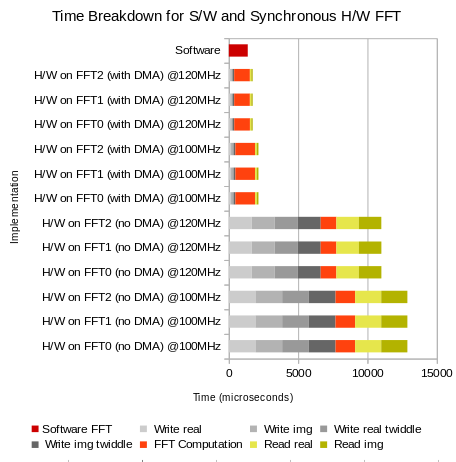
\includegraphics[width=0.47\textwidth]{hw_v_sw_dma_and_no_dma}\\
\caption{Time breakdown of an FFT done in software versus in hardware, showing all implementations (with/without a DMA engine, and with peripherals clocked at 100MHz and 120MHz). Each critical step is highlighted in a different color. Copying of input operands is highlighted in shades of gray, the actual computation in shades of red, and copying back results in shades of yellow.}
\label{fig:hw_sw_all}
\end{figure}

\begin{figure}
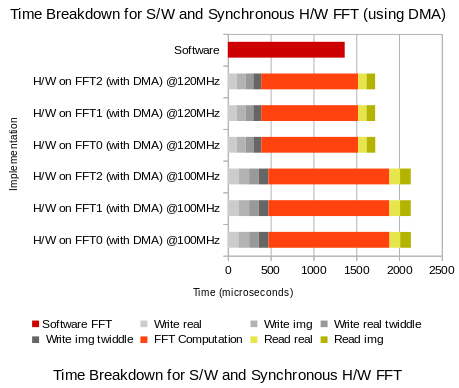
\includegraphics[width=0.47\textwidth]{hw_v_sw_dma}\\
\caption{Close-up view of execution time for the hardware implementations with a DMA engine.}
\label{fig:hw_sw_dma}
\end{figure}

Figures~\ref{fig:hw_sw_all}~and~\ref{fig:hw_sw_dma} show the time spent executing the FFT in software running entirely on the Zynq processor versus each step in hardware under different constraints. The runtime for each of the three FFT accelerators is shown at two different clock rates and with and without a DMA engine.

One will notice that using the DMA drastically speeds up execution. On average, the DMA speeds up all data transfer by approximately 16x as compared to the processor manually copying data. Unsurprisingly, the time spent computing the FFT is unaffected by the use of a DMA engine. Figure~\ref{fig:hw_sw_dma} gives a more close-up view of how the hardware accelerator with DMA compares to software.

When increasing the clock frequency of the FFT accelerator, DMA engine, and AXI interconnect from 100MHz to 120MHz, one can see that every step of the hardware implementation speeds up, whether using the DMA or not. This is because the DMA and the Zynq processor are both constrained in how fast they can transfer data by the speed of the interconnect.

Finally, it is important to note that the software implementation is faster than hardware in all cases in terms of total execution time. However, this includes the time spent copying data to and from the FFT accelerator. In Figure~\ref{fig:hw_sw_dma}, one can see that at 120MHz, the actual computation (shown in red) is completed faster in hardware than in software. The synchronous data transfer which comes before and after computation lengthens execution time such that there is no speedup over the software implementation. Transferring data asynchronously could amortize this overhead by allowing the Zynq processor to do other useful work while data is moved by a DMA.


